\documentclass{book}
\usepackage{graphicx}                              %for PNG images (pdflatex)
\usepackage[linkbordercolor={1.0 1.0 0.0}]{hyperref} %for \url tag
\usepackage{color}                                 %for defining custom colors
\usepackage{framed}                                %for shaded and framed paragraphs
\usepackage{textcomp}                              %for various symbols, e.g. Registered Mark
\usepackage{geometry}                              %for defining page size
\usepackage{longtable}                             %for breaking tables
%\usepackage{trackchanges}
%
\geometry{verbose,a4paper,tmargin=2.5cm,bmargin=2.5cm,lmargin=2.5cm,rmargin=2CM}
\hypersetup{
  pdfauthor = {},
  pdftitle = {Documentation of the Web Service based ARC Information System},
  pdfsubject = {},
  pdfkeywords = {Paper,keyword,comma-separated},
  pdfcreator = {PDFLaTeX with hyperref package},
  pdfproducer = {PDFLaTeX}
}
%
\bibliographystyle{IEEEtran}                       %a nice bibliography style
%
\def\efill{\hfill\nopagebreak}%
\hyphenation{Nordu-Grid}
\setlength{\parindent}{0cm}
\setlength{\FrameRule}{1pt}
\setlength{\FrameSep}{8pt}
\addtolength{\parskip}{5pt}
\renewcommand{\thefootnote}{\fnsymbol{footnote}}
\renewcommand{\arraystretch}{1.3}
\newcommand{\dothis}{\colorbox{shadecolor}}
\newcommand{\ngdl}{\url{http://ftp.nordugrid.org/download}~}
\definecolor{shadecolor}{rgb}{1,1,0.6}
\definecolor{salmon}{rgb}{1,0.9,1}
\definecolor{bordeaux}{rgb}{0.75,0.,0.}
\definecolor{cyan}{rgb}{0,1,1}
%
%----- DON'T CHANGE HEADER MATTER
\hyphenation{preserve-Original}
\begin{document}
\def\today{\number\day/\number\month/\number\year}

\begin{titlepage}

\begin{tabular}{rl}
\resizebox*{3cm}{!}{
\includegraphics{ng-logo.png}}
&\parbox[b]{2cm}{\textbf \it {\hspace*{-1.5cm}NORDUGRID\vspace*{0.5cm}}}
\end{tabular}

\hrulefill

%-------- Change this to NORDUGRID-XXXXXXX-NN

{\raggedleft NORDUGRID-TECH-21\par}

{\raggedleft \today\par}

\vspace*{2cm}

%%%%---- The title ----
{\centering \textsc{\Large ARC Information System}\Large \par}
\vspace*{0.5cm}
    
%%%%---- A subtitle, if necessary ----
{\centering \textit{\large Documentation and developer's guide}\large \par}
    
\vspace*{1.5cm}
%%%%---- A list of authors ----
    {\centering \large \footnote{@} \large \par}
\end{titlepage}

\tableofcontents                          %Comment if use article style
\newpage

\renewcommand{\thefootnote}{\arabic{footnote}}


\chapter{Design Overview}
\label{cha:design_overview}

\begin{figure}[ht]
 \centering{
  \scalebox{0.6}{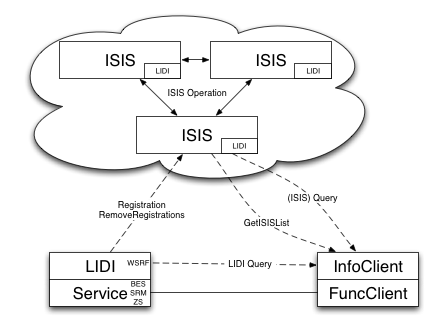
\includegraphics{SystemOverview.png}}
  \caption{\label{fig:infosys_architecture}Architecture of the Information System}
 }
\end{figure}

The Information System of the ARC middleware is composed of 3 main parts. The Information System Indexing Services (ISIS) form a set of information containers. Every generic ARC Service pushes information about itself into a nearby ISIS container/service hence registering itself to the Information System. The information stored in every ISIS is propagated among all ISIS services. Clients can query any nearby ISIS service for registered information in order to perform discovery of services that possess specific properties. Clients can also query ARC Services to obtain more detailed information about Service properties.

\chapter{ISIS}
\label{cha:isis}

\section{Registration handling}
\label{sec:isis_registration_handling}

\subsection{Functionality}
\label{sub:isis_functionality}

 The functionality of the ISIS services consists of two parts. On the one hand they are working as ordinary Web Services, and on the other hand they maintain a peer-to-peer network --- the ISIS cloud.

 The main functionality of the ISIS service visible from the outside of the ISIS cloud is to accept registrations from and provide collected information to clients. For that ISIS implements the operations described in following section.
A single ISIS service accepts Registration Records pushed to it by other services (including ISIS services) and stores them in a local XML database. Stored records can be queried by clients using mandatory and service-specific attributes as selection criteria.

 When multiple ISIS services are used they form a peer-to-peer network. Inside this cloud Registration Records are propagated between services in such a way that all ISIS instances continuously try to synchronize their databases.

% TODO: put figure here

% subsection functionality (end)

\subsection{Interface} 
\label{sub:isis_interface}

\subsubsection{Operation Register}

\begin{description}

  \item[Input]~\begin{description}
    \item[Header]~\begin{description}
      \item[RequesterID] Identifier of the client.
      \item[MessageGenerationTime] Time when the following set of RegEntries was generated. There may be multiple RegEntry elements.
    \end{description}
    \item[RegEntry]~\begin{description}
      \item[SrcAdv]~\begin{description}
        \item[Type] Type of service being registered. This element is an opaque string for now. There shall be service types defined later.
        \item[EPR] Endpoint Reference of service being registered in terms of WS-Addressing.
        \item[SSPair] Set of key/value pairs representing service specific information.
      \end{description}
      \item[MetaSrcAdv]~\begin{description}
        \item[ServiceID] Globally unique and persistent identifier of the service.
        \item[GenTime] (Generation Time) The actual timestamp of information (called wake\_up\_time in the pseudo code below)
        \item[Expiration] Validity period of Service Advertisement record.
      \end{description}
    \end{description}
  \end{description}

  \item[Output]~\begin{description}
    \item[Fault] Optional element describing fault which occurred while performing registration. If missing registration succeeded.
  \end{description}

  \item[Faults]~\begin{description}
    \item[none]No specific faults are defined
  \end{description}

\end{description}

This operation is usually called by a service that wants to register its presence in ISIS. This message consists of one or more \textbf{Registration Entries} and at most one \textbf{Registration Header}. The \textbf{Registration Entry}(RegEntry) contains a \textbf{Service Advertisement}(SrcAdv) and a corresponding \textbf{Service Advertisement Metadata}(MetaSrcAdv). This structure is shown on Figure \ref{fig:registration_message}.
\begin{figure}[ht]
\centering{{\scalebox{0.6}{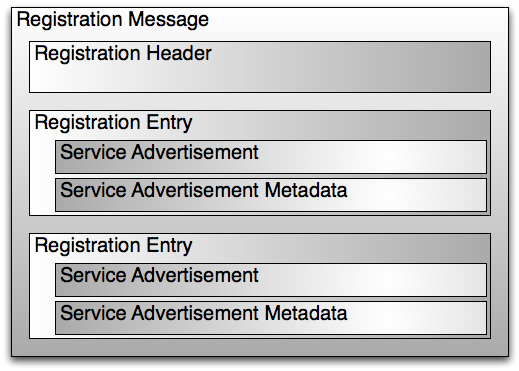
\includegraphics{RegistrationMessage.png}}}
\caption{\label{fig:registration_message}Embedded structure of Registration Message} }
\end{figure}

The service must supply mandatory information. This includes the \texttt{Endpoint Reference} used to contact the service --- the only required element is the contact URL of the service. \texttt{Type} specifies the kind of service and is used to find out functionality and interface of the service. \texttt{ServiceID} is used to distinguish between registered services and to deal with the case when the service changes its contact URL. For more information about mandatory and optional information see Section \ref{service_advertisement}.

As a result of this operation a new Registration Record is stored inside the ISIS internal database and eventually propagated to other ISISes. If a registration record with the same ID already existed it will be renewed.

This operation is also used by ISIS services to propagate Registration Records inside the ISIS cloud.

\subsubsection{Operation RemoveRegistrations}

\begin{description}

  \item[Input]~\begin{description}
    \item[MessageGenerationtime]
    \item[ServiceID] Multiple identifiers of services, whose records has to be removed.
  \end{description}

  \item[Output]~\begin{description}
    \item[RemoveRegistrationResponseElement]~\begin{description}
      \item[ServiceID] Identifier of service whose record was not removed
      \item[Fault] Description of failure reason
    \end{description}
  \end{description}

  \item[Faults]~\begin{description}
    \item[none]No specific faults are defined
  \end{description}

\end{description}

This operation is used to explicitly request the removal of zero or more Registration Entries associated with specified ServiceID values stored in the Information System. If the corresponding record does not exist its identifier will be present in the response message together with a corresponding Fault element.

\subsubsection{Operation GetISISList}

\begin{description}

  \item[Input]~\begin{description}
    \item[none]
  \end{description}

  \item[Output]~\begin{description}
    \item[EPR] Multiple Endpoint References of known ISIS services
  \end{description}

  \item[Faults]~\begin{description}
    \item[none]No specific faults are defined
  \end{description}

\end{description}

In response to this operation the EndpointReferences to all known ISIS services are returned. The operation is used for obtaining a list of known ISIS instances from any particular ISIS. Clients can then use the obtained list to run direct queries against the ISIS instances. The operation is provided for fault tolerance and for providing optional performance boost. This operation returns the known peer-to-peer neighbors. If a client is interested in all ISIS instances they can be obtained using the Query operation because they are ordinary services registered into the Information System.

\subsubsection{Operation Query}

\begin{description}

  \item[Input]~\begin{description}
    \item[QueryString] XPath query expression
  \end{description}

  \item[Output]~\begin{description}
    \item[any] Result of query
  \end{description}

  \item[Faults]~\begin{description}
    \item[none]No specific faults are defined
  \end{description}

\end{description}

This operation allows any XPath queries to be performed on stored Registration Records. The records are treated as merged in one XML document with each record being equivalent to a \texttt{RegEntry} element of a \texttt{Register} operation. In the response all elements produced by the XPath query are returned. The purpose of this operation is to make it possible to obtain any kind of information related to the Indexing Database.

% subsection interface (end)

% section registration_handling (end)

\section{Peer-to-Peer}
\label{sec:isis_peer_to_peer}

\subsection{Functionality}
\label{sub:peer_to_peer_functionality}
The ISIS nodes are able to organize themselves into a peer-to-peer network by synchronizing the stored replicated database and maintaining this synchronicity and the network topology. Every node of this peer-to-peer cloud (that is an ISIS service) has its own PeerID, an identifier only used in this network, made as a hash of its endpoint URL. The members are ordered by this identifier in a ring topology, where the successor entity of the ISIS with the largest PeerID is the ISIS with the smallest PeerID. This metric is used to define the neighbor relations that are the basis of the inter-peer-to-peer network communication. It is presumed that only registered ISIS nodes can have any role in the cloud.

\subsubsection{Connecting to the peer-to-peer network}
Every ISIS tries to connect to the network at its startup by accessing the InfoProvider ISIS nodes known from its configuration. The choice from among the few pre-configured InfoProviders is random to achieve as much load-balancing as possible. (In the design it is assumed that a huge amount of ISIS nodes are configured in very similar way, where the InfoProvider ISIS nodes are mainly the same.) If there is no InfoProvider available or nothing is known from the configuration, the node decides to be the first member and to build a new network.

If there are any InfoProvider nodes available the list of member ISIS nodes will be queried and the `successor' will be defined using the previously mentioned metric. This `successor' node will help the entering ISIS to connect to the cloud. The new member will use the `Connect' Web Service operation to get the newest version of the database stored in the peer-to-peer network, and place its own entries in the cloud by registering them. An initial database synchronization can be achieved using this method.

We can prevent the InfoProvider ISIS nodes from overloading by balancing the operation of database synchronizing --- this being the most costly procedure in the connection phase.

There is also an other extension used regarding the InfoProvider ISIS nodes. If a node is not able to connect to any of the InfoProviders then it tries to repeat it later. This results in that the network is able to fuse two disjoint parts of the network when the missing InfoProvider ISIS appears again.

\subsubsection{Routing in the peer-to-peer network}
We are keeping the databases in synch by passing every Registration and RemoveRegistrations to every node acting in the network. This yields redundancy and fault tolerant message routing between any two ISIS nodes.

The most important parameter of the network is the {\it sparsity}. This is an integer not less than 2. It determines the number of neighbors as a function of the actual number of member nodes of the network, where the number of neighbors can change when new members connect to the network or old members leave. A sparse graph can be shaped by choosing a great value for sparsity or a dense one by choosing a smaller one. This value is defined during the design and determines the main properties of the peer-to-peer network.
\begin{figure}[ht]
\centering{{\scalebox{0.6}{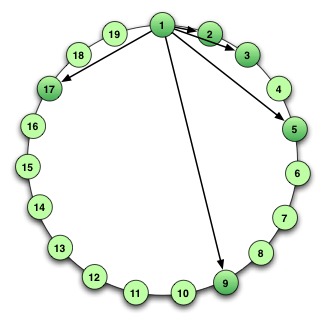
\includegraphics{Circle2-1.png}}}
\caption{\label{fig:p2p_neighbors_2} The neighbor connections in the peer-to-peer network in case of sparsity=2} }
\end{figure}

Every node has always exactly n = $\lceil \log_s{N} \rceil$ neighbors where the $N$ is the number of ISIS nodes registered into the network. The node has as many neighbors as the ISIS nodes with PeerID $s^0$-th, $s^1$-th ... $s^{n-1}$-th greater than its own. (For example: There are 19 nodes in this network with sparsity=2. Then the first node has the following neighbors: the 2nd, 3rd, 5th, 9th, and 17th node as seen in figure \ref{fig:p2p_neighbors_2}.)

There can be exactly n-way redundancy achieved in the system so at most $n-1$ node can disappear without any serious communication impair. Since there is also an emergency method used trying to deliver messages even if all neighbors are unavailable, the fault tolerance is even greater. With this extension, messages are passed to one of the non-neighbor, yet available, ISIS, so the message will surely be delivered to one of the operational node of the network. This solution provides a secure and quite fast solution for the message delivery but has a high communication cost because there are $n \times N$ messages necessary in general for every Registration or RemoveRegistrations.

If there is a much greater {\it sparsity} used, then the number of expected members decreases, in the extreme case to only one neighbor. This situation can be seen in Figure \ref{fig:p2p_neighbors_40}. In this case there are only N (the theoretically minimum) messages traversing in the network at the expense of a slower data propagation.
\begin{figure}[ht]
\centering{{\scalebox{0.6}{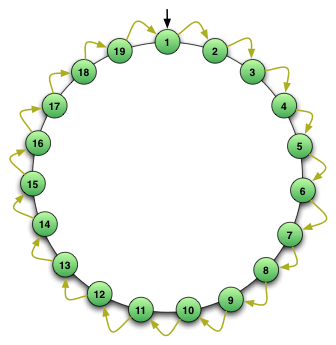
\includegraphics{Circle40-40.png}}}
\caption{\label{fig:p2p_neighbors_40} The neighbor connections in the peer-to-peer network in case of sparsity $>$ N} }
\end{figure}

There is a data-driven routing used in the peer-to-peer cloud. This means that the nodes examine the received Registration Entries and then store and forward only those messages that are newer than the already stored version belonging to the same service identifier. If the information in the message is out-of-date it will be simply dropped. (A Coordinated Universal Time (UTC) standard time and date format is used for the time stamps that is also able to handle the differences originated from the different time zones.) By using this method it is not necessary to store the formerly seen nodes in the messages, but the routing decision --- that is who to send the message to --- is based on local information. Since the routing is based on time stamps, it is very important to keep the nodes clock in synch with each other or with an outer reference, say, by using NTP.

Another advantage of this solution is the capability of handling the case of swapped Register and RemoveRegistrations messages. It is possible for a RemoveRegistrations message to forerun a previously generated Register message. This causes just a temporary imprecise entry in the database but the mistake can be quickly fixed and is not much further propagated.

Since the applied routing is based on the state of the messages belonging to some service identifier it is important to keep the fact of message deleting for a while. If a RemoveRegistrations message is received, then the named entry from the database is not removed immediately, instead its state changes to {\it deleted} and a piece of data about it (the service identifier and the deletion time) is kept.

\subsubsection{Maintenance of the peer-to-peer network}
In the network there are two different maintenance methods needed. On one hand the database has to be periodically cleaned and on the other hand the list of neighbors has always to be up-to-date.

The database applied in the system is a soft-state database so the entries are {\it valid} just for a limited time. Without any registration freshening the entry's validity will expire and its state will change to {\it expired}. The time of expiration is set in every singe message by the registrar entity. The RemoveRegistrations message turns the state of the registration entry to {\it deleted} as was previously mentioned. The {\it expired} or {\it deleted} messages will be purged in the course of periodical database maintenance. The states of registration entries are shown in Figure \ref{fig:RegEntry states}.
\begin{figure}[ht]
\centering{{\scalebox{0.6}{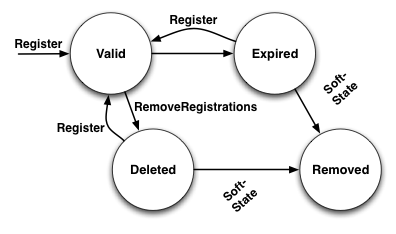
\includegraphics{RegEntryStates.png}}}
\caption{\label{fig:RegEntry states} Registration entry states} }
\end{figure}

The second kind of maintenance is keeping the list of neighbors up-to-date. While receiving Registration or RemoveRegistrations messages or when finding an outdated entry during the periodical database cleaning nodes perform the necessary steps to update the list. Since every leaving or entering node infulences the neighbor registry of all the other nodes at a high probability the local set of neighbors will be rebuilt in these cases. These modifications are passed locally because these connections are asymmetric so there is no compliance or network communication needed.

There is no special action done and no additional network traffic needed during the neighbor checking. The fact that the node periodically sends messages to every neighbor can be exploited. If the node is not successful in sending its messages to the neighbors after some tries, then the unavailable node will be marked. If every neighbor has been marked then the node changes its PeerID and reconnects to the network if there are any InfoProvider ISIS nodes available.

When a neighbor is unavailable ISIS keeps trying to deliver the message to the successor of the neighbor until either the information is passed to at least one available node or it is diagnosed that all the nodes are unavailable. Here the successor means those nodes that have greater PeerID than the neighbor but less then the next ISIS neighbor.
% subsection functionality (end)

\subsection{Interface}
\label{sub:isis_peer_to_peer_interface}
\subsubsection{Operation Connect}

\begin{description}

  \item[Input]~\begin{description}
    \item[none]
  \end{description}

  \item[Output]~\begin{description}
    \item[RegEntry] Multiple \texttt{RegEntries} locally stored in the ISIS database
  \end{description}

  \item[Faults]~\begin{description}
    \item[none]No specific faults are defined
  \end{description}

\end{description}

This operation allows the ISIS to get the already existing database from the ISIS that helps it to connect the peer-to-peer network. As a second step of the connection the newer  \texttt{RegEntries} that are stored at the connecting entity will be propagated through \texttt{Register} operation of the standard service specific interface.

% subsection interface (end)

% section peer_to_peer (end)

\section{Authorization}
\label{sec:isis_authorization}

\subsection{Client Authorization}
\label{sub:isis_authorization_client_authorization}

% TODO figure with mutiple service types

\textit{This section extensively uses terms defined in "Security Framework of ARC1" document"~\cite{arcsec}.}

To ensure that the information stored in the ISIS cloud can't be tampered with and only is available to proper clients the following authorization framework is implemented. All actions performed by ISIS clients are divided into the three following groups:

\begin{itemize}
 \item Operations initiated by other ISIS services in the cloud. Those include:
 \begin{itemize}
  \item Register with Registration Message containing information not about contacting client
  \item RemoveRegistrations with request to remove Registration Message representing not contacting client
  \item Connect indicating to provide every information about the stored database
 \end{itemize}

 Those operations may cause uncontrollable changes in collected information and must be granted only for highly trusted entities like ISISes themselves.

 \item Operations initiated by the Services registering to the Information System. Those are:
 \begin{itemize}
  \item Register with Registration Message containing information about contacting client
  \item RemoveRegistrations with request to remove Registration Message representing contacting client
 \end{itemize}

 \item Operations which are allowed for any liable client of a particular Grid infrastructure.
 \begin{itemize}
  \item Query
  \item GetISISList
 \end{itemize}
\end{itemize}

Those 3 action groups are handled using Security Framework of ARC~\cite{arcsec}. For each group a corresponding
Action is defined for the ARC policy language as described in table \ref{tab:policy_actions}.

\begin{table}[h]
\caption{ARC Policy Actions of ISIS}
\label{tab:policy_actions}
\begin{tabular}{|c|c|l|}
\hline
\textbf{Group}&\textbf{Action}&\textbf{AttributeId}\\
\hline
Request from ISIS&\textit{isis}&http://www.nordugrid.org/schemas/policy-arc/types/isis/operation\\
\hline
Request from Service&\textit{service}&http://www.nordugrid.org/schemas/policy-arc/types/isis/operation\\
\hline
Request from generic client&\textit{client}&http://www.nordugrid.org/schemas/policy-arc/types/isis/operation\\
\hline
\end{tabular}
\end{table}

Access restrictions for clients are defined using ARC Policies which are specified and 
processed using a generic Security Handlers approach. The corresponding Security Handlers have to be 
configured inside the configuration block of the corresponding ISIS service and attached to the
\textit{incoming} queue.

% subsection client_authorization (end)


\subsection{Information Authorization}
\label{sub:isis_authorization_information_authorization}

Because all ISIS services trust each other they freely exchange collected information. But 
not all information stored inside the ISIS cloud is public or readable by clients authorized according 
to the procedure described in section \ref{sub:isis_authorization_client_authorization}. There
may be some pieces of information available only for specific clients. An example could be that
information about resources serving a particular Virtual Organization (VO) might be visible only to
members of that VO.

To implement the functionality described above each node in the aggregated XML documents of information
collected by the ISIS cloud may have an Access Control Policy associated with it. Access control is 
defined at the level of an XML node and propagates to all children nodes --- similar to file systems.
Children nodes can only additionally restrict access control imposed by the parent node. For example
if parent node A allows access only to VO1 then children node B can narrow access to Administrator 
of VO1 and can't grant access for VO2 members.

By default all XML nodes are public. Access Control Policies are embedded into XML document
as XML nodes (see Appendix \ref{annex:info_policies_schema} for schema) even if that violates the schema 
of the document. Then nodes are assigned policies by adding XML attributes referring to defined Policies.
Access permission to a particular information node is evaluated by traversing all nodes from 
parent to children. At the first node that gives a negative result the evaluation is stopped and
this node including all its children is removed from document.

Before providing results of a query operation ISIS runs the procedure described above on the results and 
also removes Access Control Policies. The reduced document obtained in this way is returned to the
requesting client.

%* Clasification of information
%
% 1. From acccessibility point of view information can be devided
%into 3 groups:
% a. public
% b. available to trusted clients (like broker or scheduler service)
% c. private --- available to owner of information object and entities
%trusted by owner.
%Distinction between 2 and 3 is not clear. One may accept that 2 is
%imposed by architecture/deployment of system and 3 is controlled by
%entities which are users of the system.
% 2. From storage/access location point of view information is divided
%into:
% a. local --- stored at endpoint representing resource which is
%described by information. This information is obtainable through
%ALIS interface.
% b. propagated to dedicated services (ISIS) which collect information
%needed for pre-selection and initial lookup of services
%representing resources.
%
%NOTE: Definition of propagation of information does not exactly belong
%to security architectire of information system. But it affects it significantly
%and hence at least minimal set of definitions is needed.
%
%OUT OF BAND NOTE: Those services could provide pre-selection capability.
%
% Sets 1 and 2 may intersect in any way. In first approach to simplify
%implementation 2b may be considered to always belong to 1a.
%
%
%* Implementaion guidelines
%
% To implement set 1 information objects need to have Access Control
%Rules (ACR) assigned (usually used term Access Control List seems to
%be inadequate due to meaning of word List).
%
% To implement set 2 in similar way information objects have Propagation
%Control Rules (PCR) assigned. Because curently information system is made
%of one layer of ISIS PCRs may consist of one boolean property.
%
% Information is structured in tree-like fashion --- XML document.
%Access control is defined at node and follows all branches --- similar
%to file systems. Propagation control is similar to access control (if
%needed at all). Children nodes can't widen access defined at parent
%nodes. This should decrease amount of ACR to be evaluated.
%
%EXAMPLE: if parent node A allows access only to VO_1 then children
%node B can narrow access to Adminsitrator of VO_1 and can't open
%access for VO_2.
%
% By default all nodes are public and are propagatable. Properties
%assigned to clildren nodes limit access and propagation. Access
%permission to particular information node is evaluated by traversing
%all nodes prom parent to child. At first node which gives negative
%result evaluation is stopped.
%
% Because evaluation of permission may be costly (CPU intensive,
%causing big latency if access to external service is needed, etc.)
%other tricks to reduce cost are needed.
%
% To reduce access control evaluation cost ACRs may/should/must(?)
%be assigned to information nodes in one-to-many way --- one ACR per
%multiple information nodes. This grouping may be initiated either
%interactively (by clients explicitely specifying that same ACR is
%applicable to multiple nodes) or automatically (by comapring new
%ACR to already existing).
%
% If information nodes containing ACRs are propagated to ISIS (second
%implementation step) propagation algorithm must take ACR into account.
%For informtion propagation between ISISes this rule also applies.
%EXAMPLE: Information with access open to VO_1 must not be propagated
%to ISIS belonging to VO_2.
%
%
%** Ideas for in-memory XML documents
%
% Because informational documents are normally produced dynamically and
%have short lifetime there seems to be reasonable to keep them in memory.
% Each node with assigned ACR contains attribute (even if that breaks schema)
%containing id of ACR. ACR is defined as XML element (even if that breaks
%schema) located at higher, same or child level of considered node.
% Because informational documents are produced dynamically there are few
%ways for processing ACRs:
% 1. Right after document is generated it is traversed and ACRs applied.
%Parts of document which do not pass ACR evaluation are cut off. ACRs are
%cut off too.
% 2. While calling document generation procedure identity of client is
%supplied and ACRs are applied immediately.
% 3. While calling document generation procedure hooks/callbacks are supplied
%which are used and implement ACR evaluation.
% Combination of 1 and 3 looks most promising because it is flexible and
%keeps information system and policy evaluation code separated.
%
%
%* References
%"Information access control use cases" http://wiki.nordugrid.org/index.php/ARC1/Infosys/Access_Use_cases
%

% subsection information_authorization (end)

\subsection{Configuration}
\label{sub:isis_authorization_configuration}

\textit{For information about sophisticated authorization policies and how to deploy various Policy Decision Point entities please see "Security Framework of ARC1" document"~\cite{arcsec}.}

To restrict the set of clients allowed to perform operations on the ISIS service a proper authorization policy is needed. Let's assume ISIS is operating over a TLS connection and all participants possess X.509 certificates with the following subject names:
\begin{itemize}
\item /O=Grid/O=Test/CN=CLIENT --- generic client entities
\item /O=Grid/O=Test/CN=SERVICE --- generic service entities
\item /O=Grid/O=Test/CN=ISIS --- all ISIS belonging to ISIS cloud
\end{itemize}

\textit{In NO way do we suggest to use such setup. A real installation should use more sophisticated ways to 
identify clients contacting the ISIS service. For an infrastructure with a quite static roles distribution for 
example we suggest to use Virtual Organization Management Service (VOMS) attributes embedded into X.509 
certificates representing the participating entities.}

Below is an example policy made of 3 rules defined in lines 4--17, 18--29 and 30--39. Those define the allowed 
behavior for the ISIS, generic services and generic clients. Lines 6--7, 20--21 and 32--33 specify attributes 
used to recognise the type of the connecting client. In this case those are subjects of X.509 certificates with 
values defined above. Lines 10--15, 24--27 and 36--37 specify allowed actions. One can see that this policy 
allows all operations to be performed by the ISIS client. It limits operations allowed for generic service 
to "service" and "client" types. And client entities are allowed to perform "client" type operations only.

\begin{verbatim}
 1: <?xml version="1.0" encoding="UTF-8"?>
 2: <Policy xmlns="http://www.nordugrid.org/schemas/policy-arc" PolicyId="policy1"
 3:           CombiningAlg="Deny-Overrides">
 4:  <Rule RuleId="isis_to_isis" Effect="Permit">
 5:    <Subjects>
 6:      <Subject AttributeId="http://www.nordugrid.org/schemas/policy-arc/types/tls/identity"
 7:              >/O=Grid/O=Test/CN=ISIS</Subject>
 8:    </Subjects>
 9:    <Actions>
10:      <Action AttributeId="http://www.nordugrid.org/schemas/policy-arc/types/isis/operation"
11:             >isis</Action>
12:      <Action AttributeId="http://www.nordugrid.org/schemas/policy-arc/types/isis/operation"
13:             >service</Action>
14:      <Action AttributeId="http://www.nordugrid.org/schemas/policy-arc/types/isis/operation"
15:             >client</Action>
16:    </Actions>
17:  </Rule>
18:  <Rule RuleId="service_to_isis" Effect="Permit">
19:    <Subjects>
20:      <Subject AttributeId="http://www.nordugrid.org/schemas/policy-arc/types/tls/identity"
21:              >/O=Grid/O=Test/CN=SERVICE</Subject>
22:    </Subjects>
23:    <Actions>
24:      <Action AttributeId="http://www.nordugrid.org/schemas/policy-arc/types/isis/operation"
25:             >service</Action>
26:      <Action AttributeId="http://www.nordugrid.org/schemas/policy-arc/types/isis/operation"
27:             >client</Action>
28:    </Actions>
29:  </Rule>
30:  <Rule RuleId="client_to_isis" Effect="Permit">
31:    <Subjects>
32:      <Subject AttributeId="http://www.nordugrid.org/schemas/policy-arc/types/tls/identity"
33:              >/O=Grid/O=Test/CN=CLIENT</Subject>
34:    </Subjects>
35:    <Actions>
36:      <Action AttributeId="http://www.nordugrid.org/schemas/policy-arc/types/isis/operation"
37:             >client</Action>
38:    </Actions>
39:  </Rule>
40: </Policy>

\end{verbatim}

This policy is not as restrictive as it could be in order to allow ISIS services to register themselves as ordinary 
services and to allow services which perform discovery of other services to behave like ordinary clients.

In order to activate the policy it must be linked to the ISIS service through the Security Handle and the Policy 
Decision Point emedded into the configuration of ISIS. Below is a minimal example configuration element of 
an ISIS service. In lines 7--17 a set of Security Handlers and Policy Decision Points is configured to handle
policies written in the ARC Policy Language (described in ~\cite{arcsec}). Line 14 specifies that the policy is 
read from file \textit{/opt/arc/etc/isis/policy.xml} every time a new request arrives. If the policy is not 
satisfied then the ISIS returns SOAP Fault instead of the usual informative response.

\begin{verbatim}
 1: <Service 
 2:   xmlns="http://www.nordugrid.org/schemas/ArcConfig/2007"
 3:   xmlns:isis="http://www.nordugrid.org/schemas/ArcConfig/2009/isis"
 4:   name="isis" id="isis">
 5:  <isis:endpoint>https://localhost:60000/isis</isis:endpoint>
 6:  <isis:DBPath>/opt/arc/share/isisdb</isis:DBPath>
 7:  <SecHandler
 8:    xmlsns:auth="http://www.nordugrid.org/schemas/SimpleListAuthZ"
 9:    name="arc.authz" id="authz" event="incoming">
10:   <auth:PDP
11:     xmlns:pdp="http://www.nordugrid.org/schemas/ArcPDP"
12:     name="arc.pdp">
13:    <pdp:PolicyStore>
14:     <pdp:Location type="file">/opt/arc/etc/isis/policy.xml</pdp:Location>
15:    </pdp:PolicyStore>
16:   </auth:PDP>
17:  </SecHandler>
18: </Service>

\end{verbatim}

% subsection information_authorization (end)


% section authorization (end)

% chapter isis (end)

\chapter{Service}
\label{cha:service}

\section{Information generation}
\label{sec:service_information_generation}

The service developers have to ensure that the services are providing the necessary information about 
themselves when registering to ISISes. This is done by implementing a subclass of the Arc::Service class ---
the RegistrationCollector function has to provide up-to-date status information about the service and anything 
else it wants to be advertised. This information package is called \textbf{Service Advertisement}.
\label{service_advertisement}
The \textbf{Service Advertisement} can contain any information the service wants to advertise but the mandatory 
elements have to always be present:
\begin{itemize}
  \item Service ID: A globally unique identifier of the service.
  \item Service Type: The Glue2 type of service.
  \item Endpoint URL: The URL where the service can be contacted provided as part of EPR element.
\end{itemize}

Because there may be multiple registration processes running in parallel it is important to ensure that the
implementation of the RegistrationCollector is thread safe or there are internal locks implemented.

Every service registering to ISIS should also provide an interface for direct querying of information 
describing the service. Normally this information should be more detailed than the one sent to ISIS. For this 
purpose the LIDI interface is defined which is a subset of WS Resource Properties (WSRP)~\cite{wsrf-rp}. The following WSRP
operations must be supported --- \textit{GetResourcePropertDocument}, \textit{GetResourceProperty},
\textit{GetMultipleResourceProperties} and \textit{QueryResourceProperties}.

%TODO: define names of mandatory properties --- at least Glue2 property


% section information (end)

\section{Registration}
\label{sec:service_registration}

The registration of a service is carried out by an internal module called Registrant. The Registrant is an active module of the HED (Hosting Environment Daemon) which is bound to a set of ISISes. In practice, the configuration part of the Registrant contains exactly one ISIS to bind, and the Registrant will collect the necessary information about the other ISISes belonging to the same network.

To register services to more than one ISIS network multiple Registrant instances has to be configured. In this case, the default Registrant will be used for registering every service unless configured explicitly.
The registration of a service can be done once or periodically based either on the configuration of the Registrant or overwritten for every service separately. The Registrant is also performing message aggregation of all services linked to it if possible. The simplified algorithm of the Registrant is presented below.

\begin{framed}
  Registrant --- pseudo algorithm\\
  \\
  \verb#// Initialize phase#\\
  \verb#Read the configuration and store the information about the services in a list#\\
  \verb#do { // Cyclic phase in a different Thread#\\
  \verb# wake_up_time = now();#\\
  \verb# messages = null;#\\
  \verb#  if ( 0 < count(service where service.next_run <= wake_up_time)) {#\\
  \verb#    foreach( service where service.next_run <= wake_up_time) {#\\
  \verb#      messages.add(service.RegistrationCollector);#\\
  \verb#      service.next_run = wake_up_time + service.period;#\\
  \verb#    }#\\
  \verb#    if (0 < count(messages)) {#\\
  \verb#      sent_message = assemble message with headers(messages);#\\
  \verb#      send(sent_message);#\\
  \verb#    }#\\
  \verb#  } else {#\\
  \verb#    sleep(min(service.next_run) - now()); #\\
  \verb#  }#\\
  \verb#} while(true)#\\
\end{framed}
The current implementation does not allow the value of the period to be less than 2 minutes.

The service provides the \textbf{Service Advertisement} part of the information sent to ISIS (see Section \ref{sub:isis_interface}).
Before sending this information the Registrant extends it with additional data (\textbf{Service Advertisement Metadata}).

An example layout of services is shown on Figure \ref{fig:registration_overview}. In this configuration example 
there are two Registrants configured in one HED container for three services. The \textit{Registrant A} is the 
default Registrant and the services configured in the following way:

\begin{itemize}
  \item Service 1: There is no Registrant configured so the default one will register it.
  \item Service 2: The \textit{Registrant A} is configured explicitly.
  \item Service 3: The \textit{Registrant B} is configured explicitly.
\end{itemize}

So Service 1 and 2 are both handled by \textit{Registrant A} and Service 3 by \textit{Registrant B}.
In the first step each Registrant performs information collection from all assigned services sequentially. Registrants themselves are executing in parallel. For Figure \ref{fig:registration_overview} the approximate sequence of information collection is (\textit{A1}-\textit{A2}, \textit{B1}-\textit{B2}) followed by (\textit{A3}, \textit{A4}). After collection  the aggregated information is sent to the corresponding ISISes independently by each other Registrant (\textit{A5}, \textit{B5}).

\begin{figure}[ht]
\centering{{\scalebox{0.6}{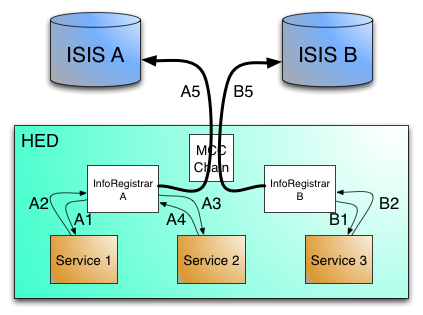
\includegraphics{Registration.png}}}
\caption{\label{fig:registration_overview}Overview of the registration process} }
\end{figure}

This registration operation is done once during the start-up phase and periodically according to 
(per service) configured periods.

% section registration (end)


\section{Authorization}
\label{sec:service_authorization}

For every piece of information provided by the service through the LIDI interface the same procedure as described in 
Section \ref{sub:isis_authorization_information_authorization} should be applied.

% section authorization (end)


\section{Configuration}
\label{sec:service_configuration}

The registration operation is done by the Registrants as described in Section \ref{sec:service_registration}.
Each Registrant is instantiated by the corresponding InfoRegistrar XML element in the configuration file as 
defined in Section \ref{annex:service_configuration_schema}. The first InfoRegistrar defines the Registrant 
that is used to register every service by default.

Registration parameters per service are defined by the InfoRegister element located inside the corresponding 
service configuration element. To assign a service to specific Registrant(s) one may use Registrar 
configuration elements situated inside InfoRegister. If no Registrar element is defined the service will 
be registered using first (default) Registrant. To make a service not register itself the special configuration element 
NoRegister has to be used.

The Following elements are defined inside the configuration element of the Registrant:
\begin{description}
\item{URL} specifies the contact endpoint of a bootstrap ISIS. If needed further ISIS addresses will be 
queried from this service. This element is mandatory.
\item{KeyPath, CertificatePath, ProxyPath and CACertificatesDir} are paths to files storing X509 
credentials used for establishing connections. Those elements are optional and needed only if 
TLS communication is used.
\item{Retry} specifies how many times communication to ISIS have to fail/timeout to start treating it
as unavailable. The default value is 5.
\end{description}

% section configuration (end)

% section configuration (end)

% chapter service (end)

\chapter{Appendices}

\section{WSDL of ISIS Specific Interface}
\label{annex:isis_wsdl}
\begin{verbatim}

?xml version="1.0" encoding="UTF-8"?>
<!--
    Data types of Information Indexing Service
-->

<xsd:schema
  xmlns:xsd="http://www.w3.org/2001/XMLSchema"
  xmlns:isis="http://www.nordugrid.org/schemas/isis/2007/06"
  xmlns:wsa="http://www.w3.org/2005/08/addressing"
  targetNamespace="http://www.nordugrid.org/schemas/isis/2007/06"
  elementFormDefault="qualified" attributeFormDefault="unqualified"
>

    <xsd:import namespace="http://www.w3.org/2005/08/addressing" schemaLocation="http://www.w3.org/2006/03/addressing/ws-addr.xsd"/>


<!-- This is an initial and incomplete DRAFT which mainly concentrates on the structure but not on the actual names. Final version will use G
LUE-2.0 ternminology. -->

    <!-- ==== Input and output types for IIS operations ==== -->
    <!-- Input type for Register operation -->
    <xsd:complexType name="RegisterType">
        <xsd:sequence>
            <xsd:element name="Header" type="isis:HeaderType" minOccurs="0" maxOccurs="1"/>
            <xsd:element name="RegEntry" type="isis:RegistrationEntryType" minOccurs="1" maxOccurs="unbounded"/>
        </xsd:sequence>
    </xsd:complexType>
    <xsd:element name="Register" type="isis:RegisterType"/>

    <!-- Output type for Register operation -->
    <xsd:complexType name="RegisterResponseType">
        <xsd:sequence>
            <xsd:element name="Fault" type="isis:FaultType" minOccurs="0" maxOccurs="1"/>
        </xsd:sequence>
    </xsd:complexType>
    <xsd:element name="RegisterResponse" type="isis:RegisterResponseType"/>

    <!-- Input type for RemoveRegistrations operation -->
    <xsd:complexType name="RemoveRegistrationsType">
        <xsd:sequence>
            <xsd:element name="MessageGenerationTime" type="xsd:string" minOccurs="1" maxOccurs="1"/>
            <xsd:element name="ServiceID" type="xsd:string" minOccurs="1" maxOccurs="unbounded"/>
        </xsd:sequence>
    </xsd:complexType>
    <xsd:element name="RemoveRegistrations" type="isis:RemoveRegistrationsType"/>

    <!-- Output type for RemoveRegistrations operation -->
    <xsd:complexType name="RemoveRegistrationResponseElementType">
        <xsd:sequence>
            <xsd:element name="ServiceID" type="xsd:string" minOccurs="1" maxOccurs="1"/>
            <xsd:element name="Fault" type="isis:FaultType" minOccurs="1" maxOccurs="1"/>
        </xsd:sequence>
    </xsd:complexType>

    <xsd:complexType name="RemoveRegistrationsResponseType">
        <xsd:sequence>
            <xsd:element name="RemoveRegistrationResponseElement" type="isis:RemoveRegistrationResponseElementType" minOccurs="0" maxOccurs="
unbounded" />
        </xsd:sequence>
    </xsd:complexType>
    <xsd:element name="RemoveRegistrationsResponse" type="isis:RemoveRegistrationsResponseType"/>

    <!-- Input type for GetISISList operation -->
    <xsd:complexType name="GetISISListType">
        <xsd:sequence>
        </xsd:sequence>
    </xsd:complexType>
    <xsd:element name="GetISISList" type="isis:GetISISListType"/>

    <!-- Output type for GetISISList operation -->
    <xsd:complexType name="GetISISListResponseType">
        <xsd:sequence>
            <xsd:element name="EPR" type="wsa:EndpointReferenceType" minOccurs="1" maxOccurs="unbounded"/>
        </xsd:sequence>
    </xsd:complexType>
    <xsd:element name="GetISISListResponse" type="isis:GetISISListResponseType"/>

    <!-- Input type for Query operation -->
    <xsd:complexType name="QueryType">
        <xsd:sequence>
            <xsd:element name="QueryString" type="xsd:string" minOccurs="1" maxOccurs="1"/>
        </xsd:sequence>
    </xsd:complexType>
    <xsd:element name="Query" type="isis:QueryType"/>
    <!-- Output type for Query operation -->
    <xsd:complexType name="QueryResponseType">
        <xsd:sequence>
            <xsd:any minOccurs="0" maxOccurs="unbounded"/>
        </xsd:sequence>
    </xsd:complexType>
    <xsd:element name="QueryResponse" type="isis:QueryResponseType"/>

    <!-- === Helper type definitions === -->
    <xsd:simpleType name="StatusType">
        <xsd:restriction base="xsd:string">
            <xsd:enumeration value="1"/>
            <xsd:enumeration value="2"/>
        </xsd:restriction>
    </xsd:simpleType>

    <xsd:complexType name="HeaderType">
        <xsd:sequence>
            <!-- Identifier of the source HED -->
            <xsd:element name="RequesterID" type="xsd:string" minOccurs="0" maxOccurs="1"/>
            <!-- Time of the aggregated message generation -->
            <xsd:element name="MessageGenerationTime" type="xsd:dateTime"/>
        </xsd:sequence>
    </xsd:complexType>

    <xsd:complexType name="RegistrationEntryType">
        <xsd:sequence>
            <xsd:element name="SrcAdv" type="isis:ServiceAdvertisementType" minOccurs="1" maxOccurs="1"/>
            <xsd:element name="MetaSrcAdv" type="isis:ServiceAdvertisementMetadataType" minOccurs="1" maxOccurs="1"/>
        </xsd:sequence>
    </xsd:complexType>

    <xsd:complexType name="ServiceAdvertisementType">
        <xsd:sequence>
            <!-- General part of the Service Advertisment -->
            <xsd:element name="Type" type="isis:ServiceTypeType"/>
            <xsd:element name="EPR" type="wsa:EndpointReferenceType"/>
            <!-- Service specific part of the Service Advertisment -->
            <xsd:element name="SSPair" type="isis:NameValuePairType" minOccurs="0" maxOccurs="unbounded"/>
        </xsd:sequence>
    </xsd:complexType>


    <xsd:complexType name="ServiceAdvertisementMetadataType">
        <xsd:sequence>
            <!-- Globally unique and persistent ID of the service -->
            <xsd:element name="ServiceID" type="xsd:string" minOccurs="1" maxOccurs="1"/>
            <!-- Time of information generation or collection -->
            <xsd:element name="GenTime" type="xsd:dateTime" minOccurs="1" maxOccurs="1"/>
            <xsd:element name="Expiration" type="xsd:duration"/>
        </xsd:sequence>
    </xsd:complexType>

    <xsd:simpleType name="FaultTypeType">
        <xsd:restriction base="xsd:string">
            <xsd:enumeration value="1"/>
            <xsd:enumeration value="2"/>
        </xsd:restriction>
    </xsd:simpleType>

    <!-- description of fault -->
    <xsd:complexType name="FaultType">
        <xsd:sequence>
            <xsd:element name="Name"        type="xsd:string"/>
            <xsd:element name="Type"        type="isis:FaultTypeType"/>
            <xsd:element name="Description" type="xsd:string"/>
        </xsd:sequence>
    </xsd:complexType>

    <!-- List of the service types will be provided by the GLUE-2.0 -->
    <xsd:simpleType name="ServiceTypeType">
        <xsd:restriction base="xsd:string">
        </xsd:restriction>
    </xsd:simpleType>

    <xsd:complexType name="NameValuePairType">
        <xsd:sequence>
            <xsd:element name="Name" type="xsd:string"/>
            <xsd:element name="Value" type="xsd:string"/>
        </xsd:sequence>
    </xsd:complexType>

</xsd:schema>


<?xml version="1.0" encoding="utf-8"?>
<wsdl:definitions name="InformationIndexing"
  xmlns:SOAP-ENV="http://schemas.xmlsoap.org/soap/envelope/"
  xmlns:SOAP-ENC="http://schemas.xmlsoap.org/soap/encoding/"
  xmlns:wsdl="http://schemas.xmlsoap.org/wsdl/"
  xmlns:xsd="http://www.w3.org/2001/XMLSchema"
  xmlns:soap="http://schemas.xmlsoap.org/wsdl/soap/"
  xmlns:wsa="http://www.w3.org/2005/08/addressing"
  xmlns:isis="http://www.nordugrid.org/schemas/isis/2007/06"
  xmlns:wsrf-bf="http://docs.oasis-open.org/wsrf/bf-2"
  xmlns:wsrf-rp="http://docs.oasis-open.org/wsrf/rp-2"
  xmlns:wsrf-rpw="http://docs.oasis-open.org/wsrf/rpw-2"
  xmlns:wsrf-rw="http://docs.oasis-open.org/wsrf/rw-2"
  targetNamespace="http://www.nordugrid.org/schemas/isis/2007/06"
>
<!--
Interface of Information Indexing Service
-->

    <wsdl:import namespace="http://docs.oasis-open.org/wsrf/rpw-2" location="http://docs.oasis-open.org/wsrf/rpw-2.wsdl"/>


    <!-- ======= Type definitions ====== -->
    <wsdl:types>
        <xsd:schema
            xmlns:isis="http://www.nordugrid.org/schemas/isis/2007/06"
            targetNamespace="http://www.nordugrid.org/schemas/isis/2007/06"
            attributeFormDefault="unqualified"
            elementFormDefault="qualified"
            >
            <xsd:include schemaLocation="./isis.xsd"/>
        </xsd:schema>
    </wsdl:types>

<!-- ====== Messages definitions ====== -->

<!-- ====== Register ====== -->
<wsdl:message name="RegisterRequest">
    <wsdl:part name="Register"  element="isis:Register"/>
</wsdl:message>

<wsdl:message name="RegisterResponse">
    <wsdl:part name="RegisterResponse" element="isis:RegisterResponse"/>
</wsdl:message>

<!-- ====== RemoveRegistrations ====== -->

<wsdl:message name="RemoveRegistrationsRequest">
    <wsdl:part name="RemoveRegistrations" element="isis:RemoveRegistrations"/>
</wsdl:message>

<wsdl:message name="RemoveRegistrationsResponse">
    <wsdl:part name="RemoveRegistrationsResponse" element="isis:RemoveRegistrationsResponse"/>
</wsdl:message>

<!-- ====== GetISISList ====== -->
<wsdl:message name="GetISISListRequest">
    <wsdl:part name="GetISISList" element="isis:GetISISList"/>
</wsdl:message>

<wsdl:message name="GetISISListResponse">
    <wsdl:part name="GetISISListResponse" element="isis:GetISISListResponse"/>
</wsdl:message>

<!-- ====== Query ====== -->
<wsdl:message name="QueryRequest">
    <wsdl:part name="Query" element="isis:Query"/>
</wsdl:message>

<wsdl:message name="QueryResponse">
    <wsdl:part name="QueryResponse" element="isis:QueryResponse"/>
</wsdl:message>

<!-- ====== PortType definitions ====== -->
<wsdl:portType name="ISISPortType">
    <wsdl:operation name="Register">
        <wsdl:input name="RegisterRequest" message="isis:RegisterRequest"/>
        <wsdl:output name="RegisterResponse" message="isis:RegisterResponse"/>
    </wsdl:operation>
    <wsdl:operation name="RemoveRegistrations">
        <wsdl:input name="RemoveRegistrationsRequest" message="isis:RemoveRegistrationsRequest"/>
        <wsdl:output name="RemoveRegistrationsResponse" message="isis:RemoveRegistrationsResponse"/>
    </wsdl:operation>
    <wsdl:operation name="GetISISList">
        <wsdl:input name="GetISISListRequest" message="isis:GetISISListRequest"/>
        <wsdl:output name="GetISISListResponse" message="isis:GetISISListResponse"/>
    </wsdl:operation>
    <wsdl:operation name="Query">
        <wsdl:input name="QueryRequest" message="isis:QueryRequest"/>
        <wsdl:output name="QueryResponse" message="isis:QueryResponse"/>
    </wsdl:operation>
</wsdl:portType>

<!-- ====== Bindings ====== -->

<wsdl:binding name="isis" type="isis:ISISPortType">
    <soap:binding style="document" transport="http://schemas.xmlsoap.org/soap/http"/>
    <wsdl:operation name="Register">
        <soap:operation soapAction="Register"/>
        <wsdl:input name="RegisterRequest">
            <soap:body use="literal"/>
        </wsdl:input>
        <wsdl:output name="RegisterResponse">
            <soap:body use="literal"/>
        </wsdl:output>
    </wsdl:operation>
    <wsdl:operation name="RemoveRegistrations">
        <soap:operation soapAction="RemoveRegistrations"/>
        <wsdl:input name="RemoveRegistrationsRequest">
            <soap:body use="literal"/>
        </wsdl:input>
        <wsdl:output name="RemoveRegistrationsResponse">
            <soap:body use="literal"/>
        </wsdl:output>
    </wsdl:operation>
    <wsdl:operation name="GetISISList">
        <soap:operation soapAction="GetISISList"/>
        <wsdl:input name="GetISISListRequest">
            <soap:body use="literal"/>
        </wsdl:input>
        <wsdl:output name="GetISISListResponse">
            <soap:body use="literal"/>
        </wsdl:output>
    </wsdl:operation>
    <wsdl:operation name="Query">
        <soap:operation soapAction="Query"/>
        <wsdl:input name="QueryRequest">
            <soap:body use="literal"/>
        </wsdl:input>
        <wsdl:output name="QueryResponse">
            <soap:body use="literal"/>
        </wsdl:output>
    </wsdl:operation>
</wsdl:binding>
<wsdl:binding name="GetResourcePropertyDocument" type="wsrf-rpw:GetResourcePropertyDocument">
    <soap:binding style="document" transport="http://schemas.xmlsoap.org/soap/http"/>
    <wsdl:operation name="GetResourcePropertyDocument">
       <soap:operation soapAction="GetResourcePropertyDocument"/>
       <wsdl:input name="GetResourcePropertyDocumentRequest">
         <soap:body use="literal"/>
        </wsdl:input>
        <wsdl:output name="GetResourcePropertyDocumentResponse">
            <soap:body use="literal"/>
        </wsdl:output>
        <wsdl:fault name="ResourceUnknownFault">
            <soap:fault name="ResourceUnknownFault" use="literal"/>
        </wsdl:fault>
        <wsdl:fault name="ResourceUnavailableFault">
            <soap:fault name="ResourceUnavailableFault" use="literal"/>
        </wsdl:fault>
    </wsdl:operation>
</wsdl:binding>

<wsdl:binding name="GetResourceProperty" type="wsrf-rpw:GetResourceProperty">
    <soap:binding style="document" transport="http://schemas.xmlsoap.org/soap/http"/>
    <wsdl:operation name="GetResourceProperty">
        <soap:operation soapAction="GetResourceProperty"/>
        <wsdl:input name="GetResourcePropertyRequest">
            <soap:body use="literal"/>
        </wsdl:input>
        <wsdl:output name="GetResourcePropertyResponse">
            <soap:body use="literal"/>
        </wsdl:output>
        <wsdl:fault name="ResourceUnknownFault">
            <soap:fault name="ResourceUnknownFault" use="literal"/>
        </wsdl:fault>
        <wsdl:fault name="ResourceUnavailableFault">
            <soap:fault name="ResourceUnavailableFault" use="literal"/>
        </wsdl:fault>
        <wsdl:fault name="InvalidResourcePropertyQNameFault">
            <soap:fault name="InvalidResourcePropertyQNameFault" use="literal"/>
        </wsdl:fault>
    </wsdl:operation>
</wsdl:binding>

<wsdl:binding name="QueryResourceProperties" type="wsrf-rpw:QueryResourceProperties">
    <soap:binding style="document" transport="http://schemas.xmlsoap.org/soap/http"/>
    <wsdl:operation name="QueryResourceProperties">
        <soap:operation soapAction="QueryResourceProperties"/>
        <wsdl:input name="QueryResourcePropertiesRequest">
            <soap:body use="literal"/>
        </wsdl:input>
        <wsdl:output name="QueryResourcePropertiesResponse">
            <soap:body use="literal"/>
        </wsdl:output>
        <wsdl:fault name="ResourceUnknownFault">
            <soap:fault name="ResourceUnknownFault" use="literal"/>
        </wsdl:fault>
        <wsdl:fault name="ResourceUnavailableFault">
            <soap:fault name="ResourceUnavailableFault" use="literal"/>
        </wsdl:fault>
        <wsdl:fault name="InvalidResourcePropertyQNameFault">
            <soap:fault name="InvalidResourcePropertyQNameFault" use="literal"/>
        </wsdl:fault>
        <wsdl:fault name="UnknownQueryExpressionDialectFault">
            <soap:fault name="UnknownQueryExpressionDialectFault" use="literal"/>
        </wsdl:fault>
        <wsdl:fault name="InvalidQueryExpressionFault">
            <soap:fault name="InvalidQueryExpressionFault" use="literal"/>
        </wsdl:fault>
        <wsdl:fault name="QueryEvaluationErrorFault">
            <soap:fault name="QueryEvaluationErrorFault" use="literal"/>
        </wsdl:fault>
    </wsdl:operation>
</wsdl:binding>

<!-- ====== Service definition ====== -->
<wsdl:service name="isis">
    <wsdl:port name="GetResourcePropertyDocument" binding="isis:GetResourcePropertyDocument">
        <soap:address location="mailto:test@test.com"/>
    </wsdl:port>
    <wsdl:port name="GetResourceProperty" binding="isis:GetResourceProperty">
        <soap:address location="mailto:test@test.com"/>
    </wsdl:port>
    <wsdl:port name="QueryResourceProperties" binding="isis:QueryResourceProperties">
        <soap:address location="mailto:test@test.com"/>
    </wsdl:port>
    <wsdl:port name="isis" binding="isis:isis">
        <soap:address location="mailto:test@test.com"/>
    </wsdl:port>
</wsdl:service>

</wsdl:definitions>
\end{verbatim}

% section isis_wsdl (end)

\section{Schema of ISIS Configuration}
\label{annex:isis_configuration_schema}
\begin{verbatim}

<?xml version="1.0" encoding="UTF-8"?>
<xsd:schema
  xmlns:xsd="http://www.w3.org/2001/XMLSchema"
  xmlns="http://www.nordugrid.org/schemas/ArcConfig/2009/isis"
  xmlns:icfg="http://www.nordugrid.org/schemas/ArcConfig/2009/isis"
  targetNamespace="http://www.nordugrid.org/schemas/ArcConfig/2009/isis"
  elementFormDefault="qualified" attributeFormDefault="unqualified"
>

  <xsd:element name="endpoint" type="xsd:anyURI"/>

  <xsd:element name="retry" type="xsd:nonNegativeInteger" minOccurs="0"/>

  <xsd:element name="sparsity" type="xsd:nonNegativeInteger" minOccurs="0"/>

  <xsd:simpleType name="Logger_Type">
    <xsd:restriction base="xsd:string"/>
    <xsd:attribute name="level" type="xsd:string" use="optional"/>
  </xsd:simpleType>
  <xsd:element name="Logger" type="icfg:Logger_Type" minOccurs="0"/>

  <xsd:element name="ETValid" type="xsd:nonNegativeInteger" minOccurs="0"/>

  <xsd:element name="ETRemove" type="xsd:nonNegativeInteger" minOccurs="0"/>

  <xsd:element name="DBPath" type="xsd:string"/>

  <xsd:complexType name="InfoProvider_Type">
    <xsd:sequence>
      <xsd:element name="URL" type="xsd:anyURI"/>
    </xsd:sequence>
  </xsd:complexType>
  <xsd:element name="InfoProvider" type="icfg:InfoProvider_Type" minOccurs="0" maxOccurs="unbounded"/>

</xsd:schema>

\end{verbatim}

% section isis_configuration_schema (end)

\section{Schema of Service Registartion Configuration}
\label{annex:service_configuration_schema}
\begin{verbatim}

<?xml version="1.0" encoding="UTF-8"?>
<xsd:schema
  xmlns:xsd="http://www.w3.org/2001/XMLSchema"
  xmlns:iregc="http://www.nordugrid.org/schemas/InfoRegisterConfig/2008"
  targetNamespace="http://www.nordugrid.org/schemas/InfoRegisterConfig/2008"
  elementFormDefault="qualified">

    <xsd:complexType name="InfoRegistrar_Type">
        <!-- This element defines configuration of Information Registration
             active element. This element is located at top level configuration
             document. Each instance if such element instatiates one instance
             of Information Registrant active element. -->
        <xsd:sequence>
            <!-- URL specifies contact endpoint of a bootstrap Information
                 Registration service. Further ISIS adresses will be queried
                 from this service. -->
            <xsd:element name="URL" type="xsd:string"/> <!-- maxOccurs="unbounded" -->
            <!-- Optional KeyPath, CertificatePath, ProxyPath and CACertificatesDir are
                 paths to files storing X509 credentials used for establishing connections. -->
            <xsd:element name="KeyPath" type="xsd:string" minOccurs="0"/>
            <xsd:element name="CertificatePath" type="xsd:string" minOccurs="0"/>
            <xsd:element name="ProxyPath" type="xsd:string" minOccurs="0"/>
            <xsd:element name="CACertificatesDir" type="xsd:string" minOccurs="0"/>
            <!-- Retry count. Specifie how many times have an ISIS to timeout to handle it as
                 unavailable. If there is no value specified the default value: 5 will be used. -->
            <xsd:element name="Retry" type="xsd:string" minOccurs="0" maxOccurs="1"/>
        </xsd:sequence>
        <!-- Attribute id may be used to refer to this element -->
        <xsd:attribute name="id" type="xsd:string" use="optional"/>
    </xsd:complexType>
    <xsd:element name="InfoRegistrar" type="iregc:InfoRegistrar_Type"/>

    <xsd:complexType name="Registrar_Type">
        <xsd:sequence>
            <!-- Missing elements means that the default values will be used. -->

            <!-- Period specifies how often registration to be done in minutes.
                 The 0 value means single registration. -->
            <xsd:element name="Period" type="xsd:nonNegativeInteger" minOccurs="0" maxOccurs="1"/>
            <!-- Element defines the unique id of the service propagated outside. -->
            <xsd:element name="ServiceID" type="xsd:string" minOccurs="0" maxOccurs="1"/>
            <!-- This element defines URL of the service as seen from outside. -->
            <xsd:element name="endpoint" type="xsd:string" minOccurs="0" maxOccurs="1"/>
            <!-- This element defines the expiration time of the information provided by the service. -->
            <xsd:element name="expiration" type="xsd:string" minOccurs="0" maxOccurs="1"/>
        </xsd:sequence>
        <!-- Attribute id is to define the previously configured InfoRegistrar to be refered -->
        <xsd:attribute name="id" type="xsd:string" use="required"/>
    </xsd:complexType>

    <xsd:complexType name="InfoRegister_Type">
    <!-- Element for Service element to link it to InfoRegistrar
         elements. It may also override some configuration parameters.
         Presence of this element means that service will be registered
         to ISISes. -->
        <xsd:sequence>
            <!-- This elements specify which registrars must be used
                 for registering services. If there is no such element
                 then registration is done using all registrars. -->
            <xsd:element name="Registrar" type="iregc:Registrar_Type" minOccurs="0" maxOccurs="unbounded"/>
            <!-- Default values for every InfoRegistrar -->

            <!-- Period specifies how often registration to be done in minutes.
                 The 0 value means single registration. -->
            <xsd:element name="Period" type="xsd:nonNegativeInteger" minOccurs="1" maxOccurs="1"/>
            <!-- Element defines the unique id of the service propagated outside. -->
            <xsd:element name="ServiceID" type="xsd:string" minOccurs="0" maxOccurs="1"/>
            <!-- This element defines URL of the service as seen from outside. -->
            <xsd:element name="endpoint" type="xsd:string" minOccurs="1" maxOccurs="1"/>
            <!-- This element defines the expiration time of the information provided by the service. -->
            <xsd:element name="expiration" type="xsd:string" minOccurs="1" maxOccurs="1"/>
        </xsd:sequence>
    </xsd:complexType>
    <xsd:element name="InfoRegister" type="iregc:InfoRegister_Type"/>

    <!-- Configuration element force skipping the Self-Registration -->
    <xsd:element name="NoRegister">
        <xsd:complexType />
    </xsd:element>

</xsd:schema>

\end{verbatim}

% section service_configuration_schema (end)

\section{Schema of Information Document Policies}
\label{annex:info_policies_schema}
\begin{verbatim}

<?xml version="1.0" encoding="UTF-8"?>
<xsd:schema
  xmlns:xsd="http://www.w3.org/2001/XMLSchema"
  xmlns:if="http://www.nordugrid.org/schemas/InfoFilter/2008"
  xmlns="http://www.nordugrid.org/schemas/InfoFilter/2008"
  xmlns:policy="http://www.nordugrid.org/schemas/policy-arc"
  targetNamespace="http://www.nordugrid.org/schemas/InfoFilter/2008"
  elementFormDefault="qualified">

    <xsd:complexType name="InfoFilterDefinition_Type">
        <!-- This element is a container for single policy element of any kind.
             Attached mandatory attribute defines identifier which is then used
             to link XML elements with defined policy.
             Currently only supported policy is one defined in
             http://www.nordugrid.org/schemas/policy-arc namespace. -->
        <xsd:any namespace="##other" processContents="lax" minOccurs="1" maxOccurs="1"/>
        <xsd:attribute name="id" type="xsd:string" use="required"/>
    </xsd:complexType>
    <xsd:element name="InfoFilterDefinition" type="if:InfoFilterDefinition_Type" minOccurs="0" maxOccurs="unbounded"/>

    <xsd:attribute name="InfoFilterTag">
        <!-- This attribute is to be used in element for which authorization
             policy to be applied. It specifies identifier of policy defined
             in InfoFilterDefinition element. -->
        <xsd:simpleType>
            <xsd:restriction base="xsd:string"/>
        </xsd:simpleType>
    </xsd:attribute>

</xsd:schema>

\end{verbatim}

% section info_policies_schema (end)

\section{Example ISIS service configuration}
\label{annex:example_isis_configuration}
\begin{verbatim}
<ArcConfig
  xmlns="http://www.nordugrid.org/schemas/ArcConfig/2007"
  xmlns:tcp="http://www.nordugrid.org/schemas/ArcMCCTCP/2007"
  xmlns:isis="http://www.nordugrid.org/schemas/isis/2008/08"
  xmlns:infosys="http://www.nordugrid.org/schemas/InfoRegisterConfig/2008"
>
  <!-- Various server settings -->
  <infosys:InfoRegistrar id="NorduGridInfosys">
    <!-- Contact and behavior details of the InfoRegsitrar element-->
    <infosys:URL><!-- Available endpoint URL of an ISIS representing the cloud --></infosys:URL>
    <infosys:Retry>4</infosys:Retry>
  </infosys:InfoRegistrar>

  <Plugins><Name>isis</Name></Plugins>

  <Chain>

    <!-- Chain configuration goes here! -->
    <Plexer name="plexer.service" id="plexer">
      <next id="isis1">^/isis1$</next>
    </Plexer>

    <Service name="isis" id="isis1">
        <isis:DBPath>
            <!-- File location where the database is locally stored -->
        </isis:DBPath>
        <isis:endpoint>
            <!-- The URL where the service can be accessed from outside -->
        </isis:endpoint>
        <isis:InfoProviderISIS>
            <isis:URL>
                <!-- The URL of one or more ISIS where the other ISIS's can be queried. -->
            </isis:URL>
        </isis:InfoProviderISIS>
        <infosys:InfoRegister>
            <infosys:Period>
                <!-- How often should the service be registered. 
                For example: PT75S for 75 seconds -->
            </infosys:Period>
            <infosys:Endpoint>
                <!-- The URL where the service can be accessed from outside -->
            <infosys:Endpoint>
            <infosys:Expiration>
                <!-- The lifetime of the RegEntry provided by the service about itself.
                For example: PT5H for 5 hours -->
            </infosys:Expiration>
            <!-- If there is no specific Registrar defined then every InfoRegistrar
             will be use used during the registration. The period of the repeating 
             registration will be the value given here in every ISIS cloud. -->
        </infosys:InfoRegister>
    </Service>
  </Chain>
</ArcConfig>

\end{verbatim}
% section example_ISIS_configuration (end)

% chapter appendices (end)


\bibliography{grid}
\end{document}
